% The comment below tells Rubber to compile the .dot files.
%
% rubber: module graphics
% rubber: rules rules.ini

\documentclass{beamer}

\usetheme{default}

\usefonttheme{structurebold}
\usepackage{helvet}
\usecolortheme{seagull}         % white on black

\usepackage[utf8]{inputenc}
\PassOptionsToPackage{hyphens}{url}\usepackage{hyperref,xspace,multicol}
\usepackage[absolute,overlay]{textpos}
\usepackage{tikz}
\usetikzlibrary{arrows,shapes,trees,shadows,positioning}
\usepackage{fancyvrb}           % for '\Verb'
\usepackage{xifthen}            % for '\isempty'

% Remember the position of every picture.
\tikzstyle{every picture}+=[remember picture]

\tikzset{onslide/.code args={<#1>#2}{%
  \only<#1>{\pgfkeysalso{#2}} % \pgfkeysalso doesn't change the path
}}

% Colors.
\definecolor{guixred1}{RGB}{226,0,38}  % red P
\definecolor{guixorange1}{RGB}{243,154,38}  % guixorange P
\definecolor{guixyellow}{RGB}{254,205,27}  % guixyellow P
\definecolor{guixred2}{RGB}{230,68,57}  % red S
\definecolor{guixred3}{RGB}{115,34,27}  % dark red
\definecolor{guixorange2}{RGB}{236,117,40}  % guixorange S
\definecolor{guixtaupe}{RGB}{134,113,127} % guixtaupe S
\definecolor{guixgrey}{RGB}{91,94,111} % guixgrey S
\definecolor{guixdarkgrey}{RGB}{46,47,55} % guixdarkgrey S
\definecolor{guixblue1}{RGB}{38,109,131} % guixblue S
\definecolor{guixblue2}{RGB}{10,50,80} % guixblue S
\definecolor{guixgreen1}{RGB}{133,146,66} % guixgreen S
\definecolor{guixgreen2}{RGB}{157,193,7} % guixgreen S

\setbeamerfont{title}{size=\huge}
\setbeamerfont{frametitle}{size=\huge}
\setbeamerfont{normal text}{size=\Large}

% White-on-black color theme.
\setbeamercolor{structure}{fg=guixorange1,bg=black}
\setbeamercolor{title}{fg=white,bg=black}
\setbeamercolor{date}{fg=guixorange1,bg=black}
\setbeamercolor{frametitle}{fg=white,bg=black}
\setbeamercolor{titlelike}{fg=white,bg=black}
\setbeamercolor{normal text}{fg=white,bg=black}
\setbeamercolor{alerted text}{fg=guixyellow,bg=black}
\setbeamercolor{section in toc}{fg=white,bg=black}
\setbeamercolor{section in toc shaded}{fg=white,bg=black}
\setbeamercolor{subsection in toc}{fg=guixorange1,bg=black}
\setbeamercolor{subsection in toc shaded}{fg=white,bg=black}
\setbeamercolor{subsubsection in toc}{fg=guixorange1,bg=black}
\setbeamercolor{subsubsection in toc shaded}{fg=white,bg=black}
\setbeamercolor{frametitle in toc}{fg=white,bg=black}
\setbeamercolor{local structure}{fg=guixorange1,bg=black}

\newcommand{\highlight}[1]{\alert{\textbf{#1}}}

\title{Optimized \& Reproducible HPC Software Deployment}
\subtitle{... with GNU~Guix and free software}

\author{Pjotr Prins\footnote{UMC Utrecht, UTHSC GeneNetwork.org} \& Ludovic Courtès\footnote{Inria}}
\date{\small{FOSDEM, February 2017}}

\setbeamertemplate{navigation symbols}{} % remove the navigation bar

\AtBeginSection[]{
  \begin{frame}
    \frametitle{}
    \tableofcontents[currentsection]
  \end{frame} 
}


\newcommand{\screenshot}[2][width=\paperwidth]{
  \begin{frame}[plain]
    \begin{tikzpicture}[remember picture, overlay]
      \node [at=(current page.center), inner sep=0pt]
        {\includegraphics[{#1}]{#2}};
    \end{tikzpicture}
  \end{frame}
}


\begin{document}

\maketitle

\setbeamercolor{normal text}{bg=guixblue2}
\begin{frame}
  \Huge{\textbf{Recipe for a contemporary HPC cluster environment.}}
\end{frame}
\setbeamercolor{normal text}{fg=white,bg=black}

% https://www.plafrim.fr/en/the-platform/software-documentation/
\begin{frame}[plain]
  \Huge{\#1. Start with an old \& inflexible distro.}
\end{frame}

\begin{frame}[plain]
  \Huge{\#2. Add a layer of home-made ``modules''.}
\end{frame}

\setbeamercolor{normal text}{fg=black,bg=white}
\screenshot{images/environment-modules}
\setbeamercolor{normal text}{fg=white,bg=black}

\begin{frame}[plain]
  \LARGE{\#2b. Tweak the modules.
  \uncover<2->{\\\#2c. Oh, run-time linker error!}
  \uncover<3->{\\\#2d. Tweak build flags for user A.}
  \uncover<4->{\\\#2e. New versions are out, rebuild!}
  \uncover<5->{\\\#2f. User B unhappy cuz we upgraded.  Ignore?}
  \uncover<6->{\\...}}
\end{frame}

\begin{frame}[plain]
  \Huge{\#3. Spice up with user-built software!}
\end{frame}


\setbeamercolor{normal text}{bg=white}
\screenshot[width=0.9\paperwidth]{images/package-managers-cropped}

%% \begin{frame}[plain]
%%   \begin{tikzpicture}[remember picture, overlay]
%%     \node [at=(current page.center), inner sep=0pt]
%%           {\includegraphics[height=\paperheight]{images/universal_install_script}};
%%     \node [at=(current page.north east), anchor=south east, rotate=90,
%%            text=black, text opacity=1, fill=white, opacity=.6]{
%%       \url{http://xkcd.com/1654/}
%%     };
%%   \end{tikzpicture}
%% \end{frame}

\setbeamercolor{normal text}{bg=guixblue2}
\begin{frame}
  \Huge{\textbf{Fixing HPC cluster environments.}}
\end{frame}

\setbeamercolor{normal text}{bg=white}
\begin{frame}[plain]
  \begin{tikzpicture}[overlay]
    \node [at=(current page.center), anchor=south,
      fill=white, text width=\paperwidth, text centered,
      text height=0.5\paperheight]
          {
\includegraphics[width=0.5\paperwidth]{images/easybuild}};

          % https://github.com/LLNL/spack/blob/develop/share/spack/logo/spack-logo-text-64.png
          % https://github.com/LLNL/spack/blob/develop/share/spack/logo/spack-logo-white-text-48.png
    \node [at=(current page.center), anchor=north,
      fill=white, text width=\paperwidth, text centered,
      inner sep=0.2\paperheight]
          {
\includegraphics[width=0.4\paperwidth]{images/spack}};
  \end{tikzpicture}
\end{frame}

\screenshot[width=\paperwidth]{images/easybuild-bug}
\screenshot[width=\paperwidth]{images/spack-bug}

\setbeamercolor{normal text}{bg=guixdarkgrey}
\begin{frame}[plain]
  \Huge{\textbf{Give up on packaging?}}
  \\[1.0cm]
  \uncover<2->{\Large{$\rightarrow$ ``app bundles'' (Docker images \& co.)}}
\end{frame}
\setbeamercolor{normal text}{bg=black}

%% \setbeamercolor{normal text}{bg=guixred3,fg=white}
%% \begin{frame}[plain]
%%   \begin{quotation}
%%     \noindent
%%     \LARGE{``Debian and other distributions are going to be \textbf{that
%%         thing you run docker on}, little more.''}
%%   \end{quotation}
%%   \hfill{--- Jos Poortvliet, ownCloud developer}

%%   \begin{tikzpicture}[overlay]
%%     \node [at=(current page.south east), anchor=south east]{
%%       \url{http://lwn.net/Articles/670566/}
%%     };
%%   \end{tikzpicture}
%% \end{frame}

%% \setbeamercolor{normal text}{bg=white}
%% \begin{frame}[plain]
%%   \begin{tikzpicture}[remember picture, overlay]
%%     \node [at=(current page.center), inner sep=0pt]
%%           {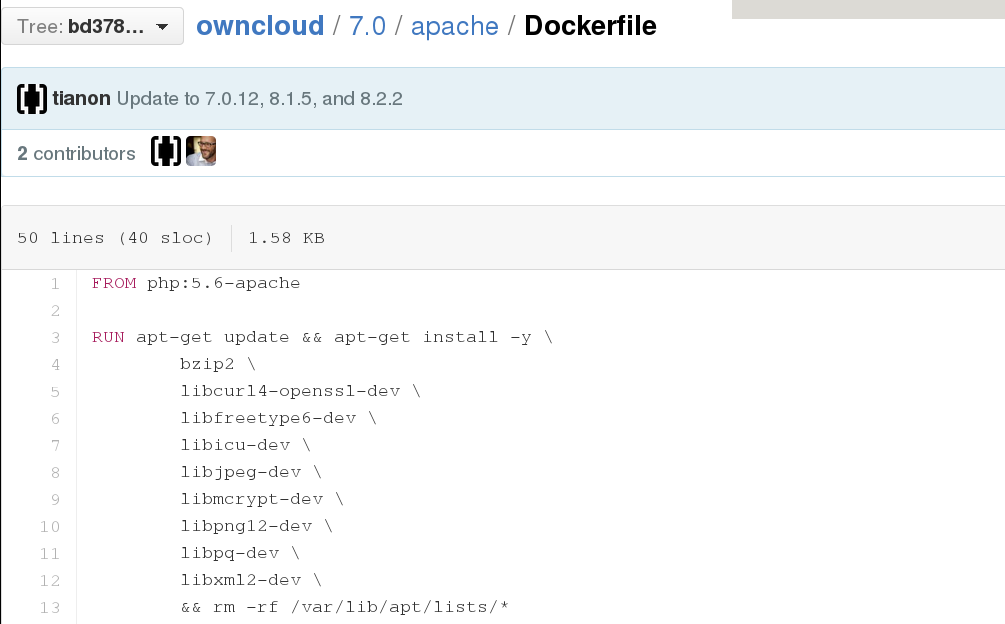
\includegraphics[height=\paperheight]{images/dockerfile-owncloud-cropped}};

%%     \node [at=(current page.center), anchor=south west, overlay,
%%            text=black, text opacity=1, fill=white, opacity=.7, text width=5cm]
%%           {\LARGE{It's also that thing you run \emph{inside} Docker!}};
%%   \end{tikzpicture}
%% \end{frame}


\setbeamercolor{normal text}{bg=white}
\begin{frame}[plain]
  \begin{tikzpicture}[remember picture, overlay]
    \node [at=(current page.center), inner sep=0pt]
          {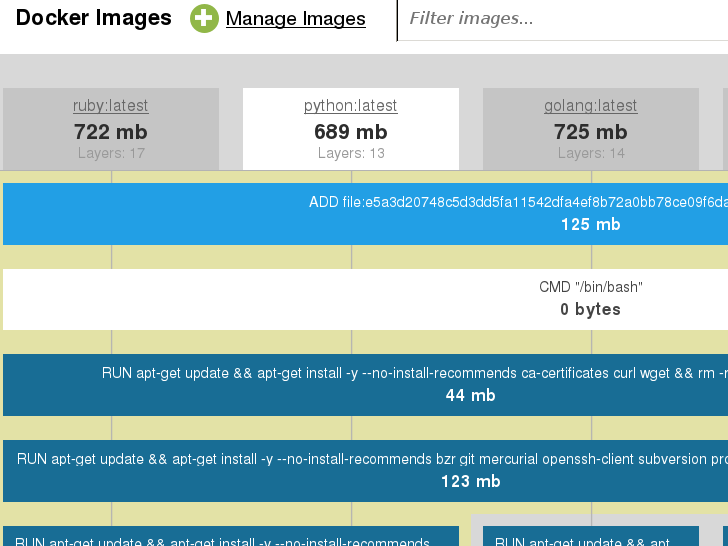
\includegraphics[width=\paperwidth]{images/docker-image-layers-cropped}};
    \node [at=(current page.north east), anchor=north east,
           text=black, text opacity=1, fill=white, opacity=.6]{
      \url{https://imagelayers.io/}
    };
  \end{tikzpicture}
\end{frame}

%% \screenshot{images/frozen-pizza}
%% \begin{frame}[plain]
%%   \begin{tikzpicture}[remember picture, overlay]
%%     \node [at=(current page.center), inner sep=0pt]
%%           {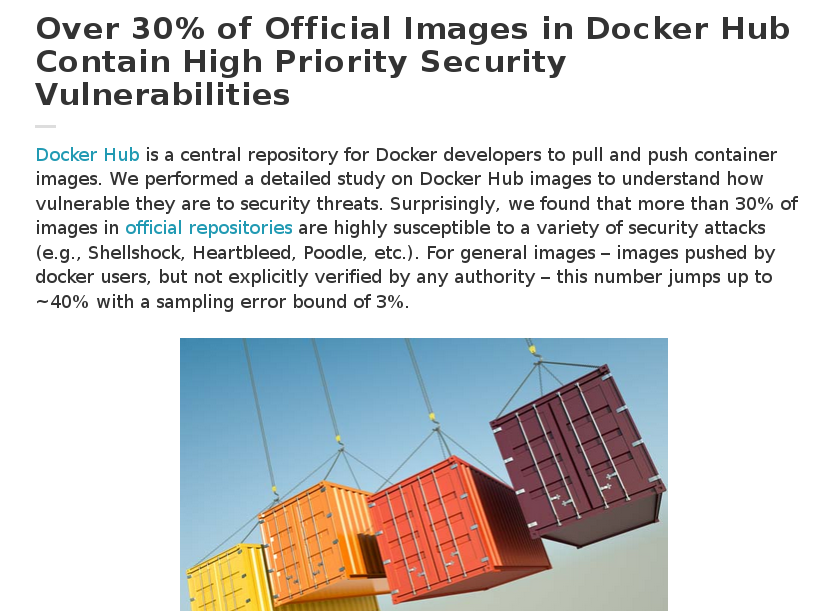
\includegraphics[height=\paperheight]{images/docker-security}};
%%     \node [at=(current page.south east), anchor=south east,
%%            text=black, text opacity=1, fill=white]{
%%       \small{\url{https://www.banyanops.com/blog/analyzing-docker-hub/}}
%%     };
%%     \node [at=(current page.south west), anchor=south west,
%%            text=black, text opacity=1, fill=white]{
%%       \small{May 2015}
%%     };
%%   \end{tikzpicture}
%% \end{frame}

\begin{frame}[plain]
  \begin{tikzpicture}[remember picture, overlay]
    \node [at=(current page.center), inner sep=0pt]
          {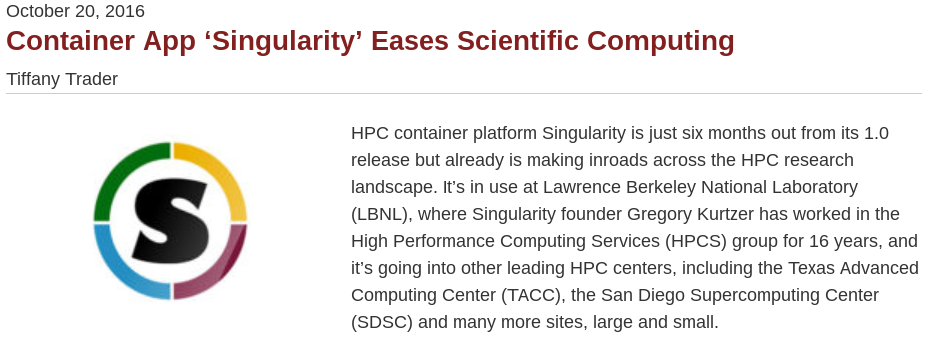
\includegraphics[width=0.95\paperwidth]{images/singularity-hpc-wire}};
    \node [at=(current page.south east), anchor=south east,
           text=black, text opacity=1, fill=white]{
      \tiny{\url{https://www.hpcwire.com/2016/10/20/singularity-containers-easing-scientific-computing}}
    };
  \end{tikzpicture}
\end{frame}

\setbeamercolor{normal text}{bg=black}
\begin{frame}[plain]{``app bundles'' are headed wrong}
  \Large{
    \begin{itemize}
    \item difficulty to \highlight{compose} software packages
    \item wrong \highlight{abstraction level}: image vs. package
    \item \highlight{hardly reproducible}: we have the bits, not the
      source
    \item makes it hard to \highlight{customize \& experiment}
    \end{itemize}
  }
\end{frame}

\setbeamercolor{normal text}{bg=white}
\begin{frame}[plain]
  \begin{tikzpicture}[remember picture, overlay]
    \node [at=(current page.center), inner sep=0pt]
          {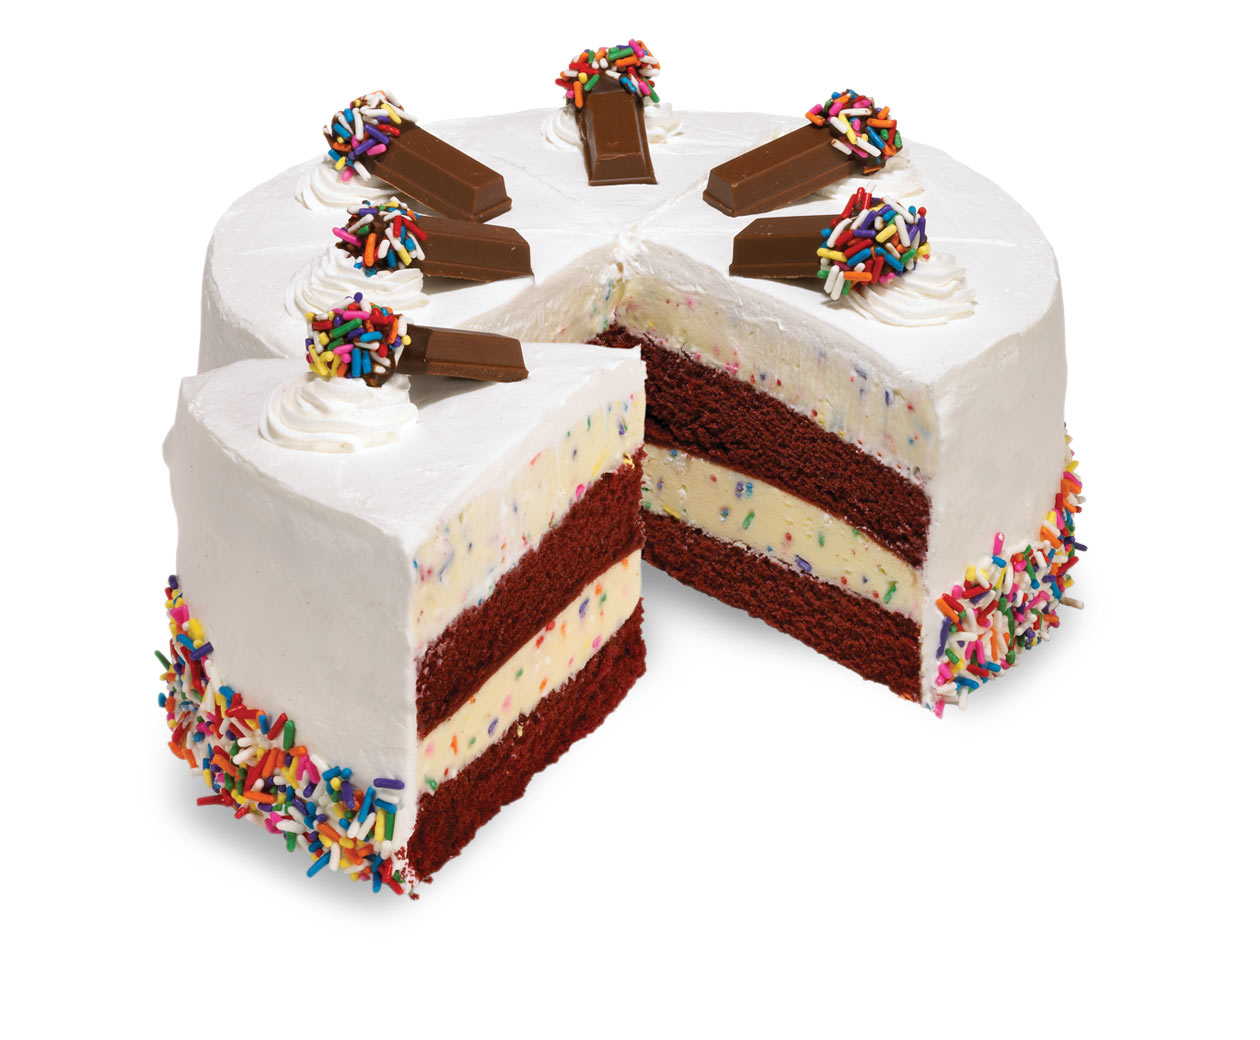
\includegraphics[height=\paperheight]{images/cake}};
    \node [at=(current page.center), anchor=north, text=black,
           fill=white, opacity=0., text opacity=1.,
           rounded corners=2mm, inner sep=1.5cm]{
      \Huge{\textbf{Can we eat it too?}}
    };
  \end{tikzpicture}
\end{frame}
\setbeamercolor{normal text}{bg=black}


%%%%%%%%%%%%%%%%%%%%%%%%%%%%%%%%%%%%%%%%%%%%%%%%%%%%%%%%%%%%%%%%%%%%%%%%%%%%%%
\setbeamercolor{normal text}{bg=white}
\begin{frame}[plain]
  \begin{tikzpicture}[remember picture, overlay]
    \node [at=(current page.center), inner sep=0pt]
          {
\includegraphics[width=0.7\paperwidth]{images/Guix-horizontal-print}};
  \end{tikzpicture}
\end{frame}
\setbeamercolor{normal text}{fg=white,bg=black}

\begin{frame}
  \LARGE{
    \begin{enumerate}
    \item transactional package manager
    \item software environment manager
    \item APIs \& tools to customize environments
    \item packaging tools
    \end{enumerate}
  }
\end{frame}

\begin{frame}
  \Large{
  \begin{itemize}
    \item started in 2012
    \item \highlight{4,800+ packages}, all free software
    \item \highlight{4 architectures}:\\
      x86\_64, i686, ARMv7, mips64el
    \item binaries at \url{https://hydra.gnu.org}
    \item 0.12.0 released in December 2016
  \end{itemize}
  }
\end{frame}

\begin{frame}{cluster deployments}
  \Large{
    \begin{itemize}
      % http://zvfak.blogspot.ch/2015/07/gnu-guix-for-easily-managing.html
    \item \highlight{Max Delbrück Center} (DE): 250-node cluster +
      workstations
      % https://ubc.uu.nl/infrastructure/
      % https://wiki.bioinformatics.umcutrecht.nl/pub/HPC/WebHome/HPC_Flyer.png
    \item \highlight{Utrecht Bioinformatics Center} (NL): 68-node
      cluster (1,000+ cores)
      % https://www.qriscloud.org.au/support/qriscloud-documentation/75-euramoo-datasheet
      % https://www.qriscloud.org.au/support/qriscloud-documentation/76-flashlite-datasheet
    \item \highlight{University of Queensland} (AU): 20-node cluster
      (900 cores)
    \item<2-> \emph{more to come!}
    \end{itemize}
  }
\end{frame}

\setbeamercolor{normal text}{bg=white}
\screenshot[width=.9\paperwidth]{images/openhub-activity}
\screenshot[width=.9\paperwidth]{images/openhub-contributors}
\setbeamercolor{normal text}{bg=black}

\begin{frame}[fragile]

  \begin{semiverbatim}
\$ guix package -i gcc-toolchain openmpi hwloc
\textrm{...}

\$ eval `guix package --search-paths`
\textrm{...}

\$ guix package --manifest=my-software.scm
\textrm{...}
  \end{semiverbatim}

  %% \begin{tikzpicture}[overlay]
  %%   \node[rounded corners=4, text centered,
  %%         fill=guixorange1, text width=3cm,
  %%         inner sep=3mm, rotate=5, opacity=.75, text opacity=1,
  %%         drop shadow={opacity=0.5}] at (5, 4) {
  %%           \textbf{\large{demo}}
  %%         };
  %% \end{tikzpicture}
\end{frame}

%% \setbeamercolor{normal text}{bg=guixdarkgrey,fg=guixred3}
%% \begin{frame}[fragile]
%%   \Huge{Want to get started hacking on hwloc?}
%%   \\[2cm]
%%   \uncover<2->{\Large{A simple matter of installing the deps, right?}}
%% \end{frame}

%% \setbeamercolor{normal text}{bg=white}
%% \begin{frame}[plain]
%%   \begin{tikzpicture}[remember picture, overlay]
%%     \node [at=(current page.center), inner sep=0pt]
%%           {\includegraphics[height=\paperheight]{images/hwloc-graph}};
%%   \end{tikzpicture}
%% \end{frame}
%% \setbeamercolor{normal text}{fg=white,bg=black}


\begin{frame}[fragile]
  %% \frametitle{Bit-Reproducible Builds$^*$}
  %% \framesubtitle{$^*$ almost!}

  \begin{semiverbatim}
\$ guix build hello
\uncover<2->{/gnu/store/\tikz[baseline]{\node[anchor=base](nixhash){\alert<2>{h2g4sf72\textrm{...}}};}-hwloc-1.11.2}

\uncover<3->{\$ \alert<3>{guix gc --references /gnu/store/\textrm{...}-hwloc-1.11.2}
/gnu/store/\textrm{...}-glibc-2.24
/gnu/store/\textrm{...}-gcc-4.9.3-lib
/gnu/store/\textrm{...}-hwloc-1.11.2
}
  \end{semiverbatim}

  \begin{tikzpicture}[overlay]
    \node<1>(labelnixhash) [fill=white, text=black, inner sep=0.5cm,
       rounded corners] at (current page.center) {%
      \Large{\textbf{isolated build}: chroot, separate name spaces, etc.}
    };

    \node<2>(labelnixhash) [fill=white, text=black] at (4cm, 2cm) {%
      hash of \textbf{all} the dependencies};
    \path[->]<2>(labelnixhash.north) edge [bend left, in=180, out=-45] (nixhash.south);

    \draw<4-> (-10pt, 105pt) [very thick, color=guixorange2, rounded corners=8pt]
      arc (10:-50:-50pt and 110pt);
    \node<4->[fill=white, text=black, text opacity=1, opacity=.7,
          rounded corners=2mm, inner sep=5mm]
      at (7, 2) {\textbf{\Large{(nearly) bit-identical for everyone}}};
  \end{tikzpicture}

\end{frame}

\setbeamercolor{normal text}{bg=white}
\begin{frame}[plain]
  \begin{tikzpicture}[remember picture, overlay]
    \node [at=(current page.center), inner sep=0pt]
          {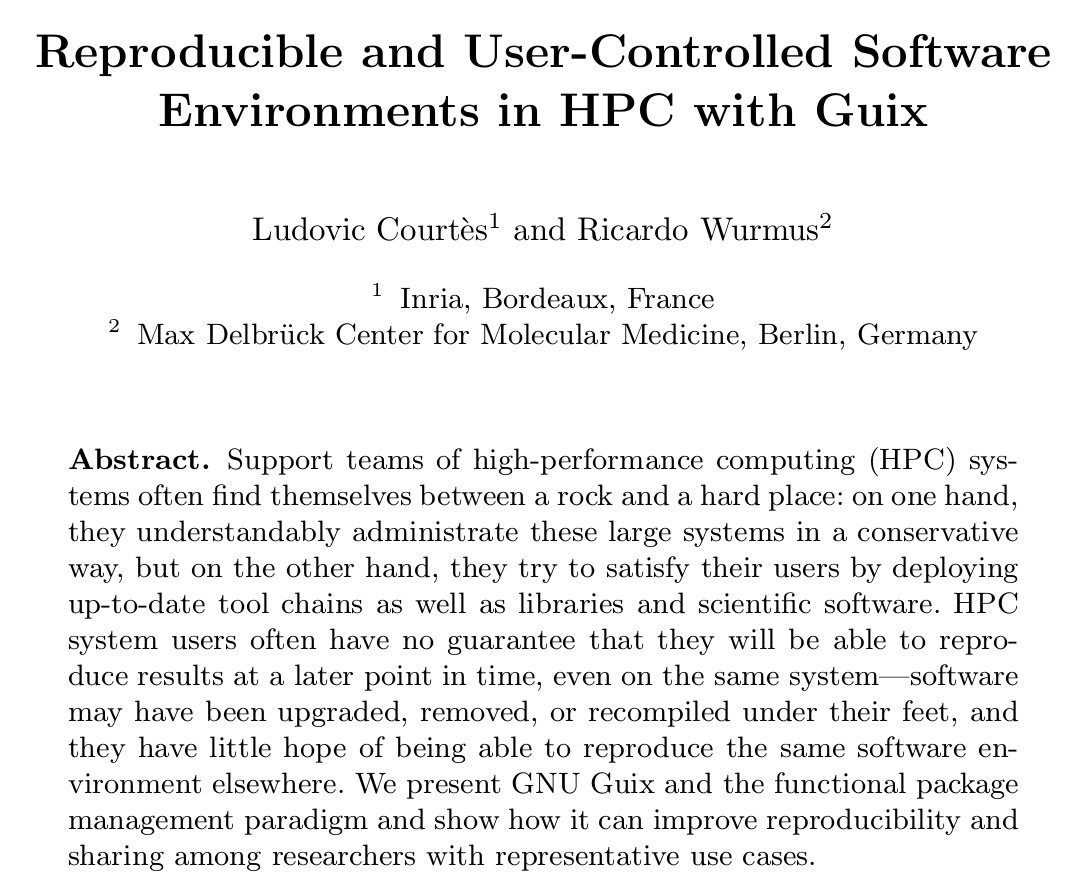
\includegraphics[height=0.8\paperheight]{images/reppar-front-page}};
    \node [at=(current page.south east), anchor=south east,
           text=black, text opacity=1, fill=white, opacity=.6]{
      \url{https://hal.inria.fr/hal-01161771/en}
    };
  \end{tikzpicture}
\end{frame}
\setbeamercolor{normal text}{fg=white,bg=black}

\begin{frame}[plain]
  \Huge{Creating package variants at the command line}
\end{frame}

\begin{frame}[fragile]
  \begin{semiverbatim}
\$ guix build hwloc \\
    \alert<1>{--with-source}=./hwloc-42.0rc1.tar.gz
\textrm{...}

\pause
\$ guix package -i mumps \\
     \alert<2>{--with-input}=scotch=pt-scotch
\textrm{...}

  \end{semiverbatim}
\end{frame}

\begin{frame}[plain]
  \Huge{Your personal packages or variants in
    \texttt{GUIX\_PACKAGE\_PATH}!}
\end{frame}

%%%%%%%%%%%%%%%%%%%%%%%%%%%%%%%%%%%%%%%%%%%%%%%%%%%%%%%%%%%%%%%%%%%%%%%%%%%%%%%%

\setbeamercolor{normal text}{bg=guixblue2}
\begin{frame}
  \Huge{\textbf{HPC \& non-root usage.}}
\end{frame}
\setbeamercolor{normal text}{fg=white,bg=black}

\begin{frame}[fragile]{}
  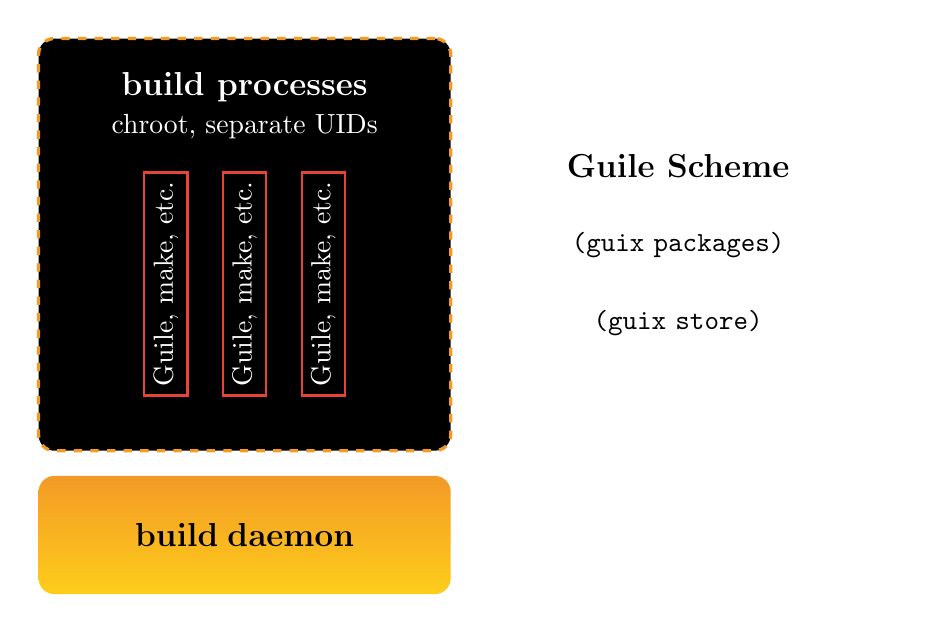
\begin{tikzpicture}[tools/.style = {
                        text width=35mm, minimum height=4cm,
                        text centered,
                        rounded corners=2mm,
                        fill=white, text=black
                      },
                      tool/.style = {
                        fill=white, text=black, text width=3cm,
                        text centered
                      },
                      daemon/.style = {
                        rectangle, text width=50mm, text centered,
                        rounded corners=2mm, minimum height=15mm,
                        top color=guixorange1,
                        bottom color=guixyellow,
                        text=black
                      },
                      builders/.style = {
                        draw=guixorange1, very thick, dashed,
                        fill=black, text=white, text width=5cm,
                        rounded corners=2mm,
                      },
                      builder/.style = {
                        draw=guixred2, thick, rectangle,
                        fill=black, text=white,
                        rotate=90
                      }]
    \matrix[row sep=3mm, column sep=1cm] {
      \node(builders)[builders, text height=5cm]{}
          node[fill=black, text=white] at (0, 2) {\large{\textbf{build processes}}}
          node[fill=black, text=white] at (0, 1.5) {chroot, separate UIDs}
          node[builder] at (-1,-0.5) {\alert{Guile}, make, etc.}
          node[builder] at ( 0,-0.5) {\alert{Guile}, make, etc.}
          node[builder] at ( 1,-0.5) {\alert{Guile}, make, etc.}; &
      \node[tools]{}
          node[fill=white, text=black] at (0, 1) {\large{\textbf{Guile Scheme}}}
          node[tool] at (0, 0) {\texttt{(guix packages)}}
          node(client)[tool] at (0, -1) {\texttt{(guix store)}};
      \\

      \node(daemon)[daemon]{\large{\textbf{build daemon}}}; &
      &
      \\
    };
  \end{tikzpicture}

  \begin{tikzpicture}[overlay]
    \path[very thick, draw=guixorange1]
      (client.south) edge [out=-90, in=0, ->] node[below, sloped]{RPCs} (daemon.east);
    \path[->, very thick, draw=guixorange1]
      (daemon) edge (builders);
  \end{tikzpicture}
\end{frame}

\begin{frame}{Allowing for non-root usage}

  \Large{
    \begin{enumerate}
      \setcounter{enumi}{-1}
    \item {run build daemon \highlight{as non-root}
      \begin{itemize}
        \item<2-> not reproducible
        \item<2-> prevents use of pre-built binaries
    \end{itemize}}
    \item {rely on Linux ``\highlight{user namespaces}''
      \begin{itemize}
        \item<3-> awesome!
        \item<3-> ... but support is missing on some systems
    \end{itemize}}
    \item make binaries \highlight{relocatable}
    \end{enumerate}
  }
\end{frame}

\setbeamercolor{normal text}{bg=guixblue2}
\begin{frame}
  \Huge{\textbf{Relocatable binaries.}}
\end{frame}
\setbeamercolor{normal text}{fg=white,bg=black}

%% \begin{frame}{The stated problem}
%% \begin{itemize}
%% \item HPC environments generally run old software (kernel, glibc, build tools)
%% \item Newer software is installed through other routes
%% \item Software targeting architectures such as Intel PHI require cross compilation
%% \end{itemize}
%% \end{frame}

%% \begin{frame}{Supercomputer}
%% \begin{itemize}
%% \item \emph{Propriety} Intel/NVIDIA/Oracle software is up-to-date
%% \item Python, R, gcc and llvm tend to be out of date
%% \item Modern languages Dlang, Go, Julia are not supported
%% \item Also Openblas and OpenCL libraries may not be supported
%% \item True on most HPC systems
%% \end{itemize}
%% \end{frame}

%% \begin{frame}{FOSS}
%% \begin{itemize}
%% \item We are FOSS people - we want recent FOSS tools - how do we cope?
%% \item Docker? Brew? Conda? From source?
%% \item And, yes, we want reproducibility too
%% \end{itemize}
%% \end{frame}

%% \begin{frame}{GNU Guix on HPC}
%% \begin{itemize}
%% \item Guix installs in a root mounted /gnu/store ...
%% \item Allow for running a privileged Guix daemon?
%% \item Perhaps allow for a mounted /gnu/store?
%% \item If not, what to do?
%% \item Answer: relocatable Guix
%% \end{itemize}
%% \end{frame}

\begin{frame}[fragile]{Insight 1}
  The first key insight: Guix store paths provide unique fingerprints:

\small
\begin{verbatim}
/gnu/store/m9vxvhdj691bq1f85lpflvnhcvrdilih-glibc-2.23/lib/libc.so
\end{verbatim}
\end{frame}

\begin{frame}[fragile]{Linked libraries}
  \small
ldd `which ldc2`
\begin{verbatim}
libconfig.so.9  /gnu/store/1v4an...-libconfig-1.5/lib/libconfig.so.9
librt.so.1      /gnu/store/m9vxv...-glibc-2.23/lib/librt.so.1
libdl.so.2      /gnu/store/m9vxv...-glibc-2.23/lib/libdl.so.2
libpthread.so.0 /gnu/store/m9vxv...-glibc-2.23/lib/libpthread.so.0
libz.so.1       /gnu/store/5992i...-zlib-1.2.8/lib/libz.so.1
libm.so.6       /gnu/store/m9vxv...-glibc-2.23/lib/libm.so.6
libstdc++.so.6  /gnu/store/9nifw...-gcc-4.9.3-lib/lib/libstdc++.so.6
libgcc_s.so.1   /gnu/store/9nifw...-gcc-4.9.3-lib/lib/libgcc_s.so.1
libc.so.6       /gnu/store/m9vxv...-glibc-2.23/lib/libc.so.6
                /gnu/store/m9vxv...-glibc-2.23/lib/ld-linux-x86-64.so.2
\end{verbatim}
\end{frame}

\begin{frame}{Relocate}
\begin{itemize}
\item Guix binaries have unique fingerprints for PATHs
\item Replace these with the target prefix
\item Only dependency is the kernel
\end{itemize}
\end{frame}


\begin{frame}[fragile]{After relocation}
  \small
  ldd $\sim$/opt/ldc-test/ldc-1.1.0-pk9rkm4zvdp6pglam7s2/bin/ldc2
\begin{verbatim}
qlibconfig.so.9  ~/opt/ldc-test/libconfig-1.5-1v4anv1.../lib/libconfig.so.9
librt.so.1      ~/opt/ldc-test/glibc-2.23-m9vxvh.../lib/librt.so.1
libdl.so.2      ~/opt/ldc-test/glibc-2.23-m9vxvh.../lib/libdl.so.2
libpthread.so.0 ~/opt/ldc-test/glibc-2.23-m9vxvh.../lib/libpthread.so.0
libz.so.1       ~/opt/ldc-test/zlib-1.2.8-5992iq1.../lib/libz.so.1
libm.so.6       ~/opt/ldc-test/glibc-2.23-m9vxvh.../lib/libm.so.6
libstdc++.so.6  ~/opt/ldc-test/gcc-4.9.3-lib-9nifwk7.../lib/libstdc++.so.6
libgcc_s.so.1   ~/opt/ldc-test/gcc-4.9.3-lib-9nifwk7.../lib/libgcc_s.so.1
libc.so.6       ~/opt/ldc-test/glibc-2.23-m9vxvh.../lib/libc.so.6
                ~/opt/ldc-test/glibc-2.23-m9vxvh.../lib/ld-linux-x86-64.so.2
\end{verbatim}
\end{frame}

\begin{frame}{What really happened here?}

  \begin{itemize}
  \item All Guix packages are isolated in the store
  \item Path is a fingerprint, e.g. \texttt{/gnu/store/m9vxvhdj691bq1f85lpflvnhcvrdilih-glibc-2.23}
  \item Scan all files and replace fingerprints with relative path \texttt{$\sim$/opt/ldc-test/glibc-2.23-m9vxvhdj691bq1f85lpf}
  \item First attempt by using Eelco Dolstra's Patchelf tool worked for shared libs by rewriting \texttt{RPATH} in binaries
  \end{itemize}
\end{frame}

\begin{frame}{Other files}
  \begin{itemize}
  \item Text files that reference the store can be rewritten (Ruby, Perl, bash scripts)
  \item Some formats are not zero-terminated (compiled Python and JVM files)
  \item Also in ELF files there are references that are not zero-terminated
  \item Solution: keep the file path at exactly the same length and patch all
  \end{itemize}
\end{frame}

\begin{frame}[fragile]{Insight 2}
  The second key insight: if a path gets rewritten with the exact same size
  string it will always work (unless there is encryption or some CRC checking)

\small
\begin{verbatim}
/gnu/store/m9vxvhdj691bq1f85lpflvnhcvrdilih-glibc-2.23/lib/libc.so
/home/user/opt/ldc-test/glibc-2.23-m9vxvhdj691bq1f851p/lib/libc.so
\end{verbatim}
\end{frame}


\begin{frame}{Same size patching}
  \begin{enumerate}
  \item start from store path, e.g.
    \texttt{/gnu/store/m9vxvhdj691bq1f85lpflvnhcvrdilih-glibc-2.23}
  \item reverse the contents
    \texttt{/gnu/store/glibc-2.23-m9vxvhdj691bq1f85lpflvnhcvrdilih}
  \item overwrite with prefix and shorten the HASH value to match the same size
  \texttt{/home/user/opt/ldc-test/glibc-2.23-m9vxvhdj691bq1f851p}
  \item and replace in all files
  \end{enumerate}
\end{frame}

\begin{frame}[fragile]{Example}
  So, store path
  \small
\begin{verbatim}
    /gnu/store/m9vxvhdj691bq1f85lpflvnhcvrdilih-glibc-2.23/bin/ldc2

    prefix /home/usr/opt/ldc-test/ becomes
    /home/user/opt/ldc-test/glibc-2.23-m9vxvhdj691bq1f851p/bin/ldc2

    prefix /usr/local/share/ldc-1.1.0/ becomes
    /usr/local/share/ldc-1.1.0/glibc-2.23-m9vxvhdj691bq1f8/bin/ldc2
\end{verbatim}
Note: prefix can be up to $\sim 40$ letters long
\end{frame}

\begin{frame}{So far\ldots}
  Successfully compiled and run
\begin{itemize}
\item ldc2 1.1.0: the LLVM D compiler
\item ruby 2.3.0: with ssl and nokogiri
\item sambamba: tool used in many sequencing HPCs around the world
\item more to come, including OpenCL, R, Python and Julia
\end{itemize}
\end{frame}

\begin{frame}{Cross compile}
\begin{itemize}
\item Install compilers that can cross compile binaries
\item LLVM can output C code
\item Provide GNU Guix packages for Intel PHI and NVIDIA TESLA
\item GNU Guix has elegant support for different targets, including a build farm for ARM, ...
\end{itemize}
\end{frame}


%%%%%%%%%%%%%%%%%%%%%%%%%%%%%%%%%%%%%%%%%%%%%%%%%%%%%%%%%%%%%%%%%%%%%%%%%%%%%%%%
\setbeamercolor{normal text}{bg=guixblue2}
\begin{frame}[plain]
  \Huge{\textbf{Wrap-up.}}
\end{frame}
\setbeamercolor{normal text}{fg=white,bg=black}

\begin{frame}{Future}
  Implications carry beyond HPC
  \\
  \begin{itemize}
  \item Automated builds with testing for different architectures
  \item Repository of binary packages
  \item One-click installs: download and run \texttt{install.sh}
  \item Ship software easily
  \item Talking about a holy grail\ldots
  \end{itemize}
\end{frame}

\begin{frame}{Summary}
  \Large{
    \begin{itemize}
    \item Guix supports \highlight{reproducible software environments}
    \item ... allows for \highlight{experimentation} through customization
    \item relocation allows \highlight{unprivileged} Guix usage in HPC
    \end{itemize}
  }
\end{frame}

\begin{frame}{Acknowledgements}
\small
\begin{itemize}
\item Roel Janssen (@roelj), Dennis Mungai (@Brainiarc7), and Frederick Muriithi (@fredmanglis) for helping with packaging D compilers, sambamba, Ruby packages, OpenCL etc.
%\item GNU Guix project leaders Ludovic Court\`{e}s and Ricardo Wurmus
\item The GNU and GNU Guix communities (many, many talented individuals)
\end{itemize}
\end{frame}

%%%%%%%%%%%%%%%%%%%%%%%%%%%%%%%%%%%%%%%%%%%%%%%%%%%%%%%%%%%%%%%%%%%%%%%%%%%%%%
\begin{frame}[plain]

\vfill{
  \vspace{2.5cm}
  \center{
\includegraphics[width=0.2\textwidth]{images/GuixSD}}\\[1.0cm]
  %% \texttt{ludo@gnu.org}
  \center{\alert{\url{https://gnu.org/software/guix/}}}
  \\
}
\end{frame}

\begin{frame}{}

  \begin{textblock}{12}(2, 8)
    \tiny{
      Copyright \copyright{} 2017 Pjotr Prins\\
      Copyright \copyright{} 2010, 2012--2017 Ludovic Courtès \texttt{ludo@gnu.org}.\\[3.0mm]
      GNU GuixSD logo, CC-BY-SA 4.0, \url{http://gnu.org/s/guix/graphics}

      Copyright of other images included in this document is held by
      their respective owners.
      \\[3.0mm]
      This work is licensed under the \alert{Creative Commons
        Attribution-Share Alike 3.0} License.  To view a copy of this
      license, visit
      \url{http://creativecommons.org/licenses/by-sa/3.0/} or send a
      letter to Creative Commons, 171 Second Street, Suite 300, San
      Francisco, California, 94105, USA.
      \\[2.0mm]
      At your option, you may instead copy, distribute and/or modify
      this document under the terms of the \alert{GNU Free Documentation
        License, Version 1.3 or any later version} published by the Free
      Software Foundation; with no Invariant Sections, no Front-Cover
      Texts, and no Back-Cover Texts.  A copy of the license is
      available at \url{http://www.gnu.org/licenses/gfdl.html}.
      \\[2.0mm]
      % Give a link to the 'Transparent Copy', as per Section 3 of the GFDL.
      The source of this document is available from
      \url{http://git.sv.gnu.org/cgit/guix/maintenance.git}.
    }
  \end{textblock}
\end{frame}

\end{document}

% Local Variables:
% coding: utf-8
% comment-start: "%"
% comment-end: ""
% ispell-local-dictionary: "american"
% compile-command: "rubber --pdf talk.tex"
% End:

%%  LocalWords:  Reproducibility
